%%%%%%%%%%%%%%%%%%%%%%%%%%%%%%%%%%%%%%%%%%%%%%%%%%%%%%%%%%%%%%%%%%%%%%%%%%%%%%%%
\chapter{Conclusion and Future Work}\label{ch:conclusion}
%%%%%%%%%%%%%%%%%%%%%%%%%%%%%%%%%%%%%%%%%%%%%%%%%%%%%%%%%%%%%%%%%%%%%%%%%%%%%%%%

\section{Final Conclusions}

\textcolor{red}{some text here}

\section{Future Work}

In this section we present some ideas for future works and implementation for SIMITAR. On the first section "Improoving results", we suggest approaches for improving the current results. They include calibration of some constants, finer controll of packet injection, and performance improovments. 

\subsection{Improoving results}

\subsubsection{Tool calibration}

To improve our results, the first approach is performing a deeper study on calibrating each tool, to achieve the best results possible. We can do this first adjusting some constants used by our algorithms. Some of these values will change the performance not for all but on tools that support stochastic functions for inter packet times. They are:

\begin{itemize}
	\item \texttt{DataProcessor::minimumAmountOfPackets}: SIMITAR only estimates stochastic models for inter-packet times if the number of flow packets is larger than this value. If it is smaller, we use only the constant model, for two reasons. First, because with a small sample, the accuracy estimate stochastic model is poor. Second, because we avoid the parameterization process, which can be costly in the case of linear regression. Its value today is set to 30.increasing this value, we may achieve a more reasonable performance for individual flows. 
	\item \texttt{DataProcessor::min\_time}: smallest time considered for inter-packet times. We use this value to avoid inter-packet times equals to zero due to the sniffer resolution. In that case, some of our procedures would diverge. It can change the fitting accuracy. Today, this value is $5e-8$. 
\end{itemize}

The modification of others  constants or approaches may change the performance for any type of underlying tool or API. They are:

\begin{itemize}

	\item \texttt{DataProcessor::m\_min\_on\_time}: this value controls the small ON time that a \textit{file} can have. This value  can change the precision of the generated traffic. Currently this value is $0.1$s. 

	\item \texttt{DataProcessor::m\_session\_cut\_time}: this member defines whatever a file transference still active or has ended. It defines the smallest OFF time acceptable. This value will change how many files SIMITAR will transfer per flow, and how many times it will call the underlying traffic generator. This constant may affect both computational performance and traffic realism.

	\item \textit{Control a minimum number of packets required for SIMITAR create a new flow}: This would reduce the number of flows created, improving its computational performance. Since SIMITAR manages each flow in a  different thread, it will create fewer threads, reducing overheads. This action should not impact  on throughput and scaling characteristics because few packets would be ignored. But it can increase the precision of the most significant flows since all the threads are competing each other on the Operational System. But, the number of flows created would be smaller.
	
\end{itemize}



% Para extensão do trafego gerado, é necessário um estudo da melhor calibração para cada ferramente, como o D-ITG, Iperf, Libtins, o que pode melhorar os resultados

\subsubsection{SIMITAR as a Packet Injector}

This proposed functionality is still under implementation, and we are using Libtins API \footnote{\href{http://libtins.github.io/}{http://libtins.github.io/}}. It enables packet crafting and injection at a reasonable performance, and provide support for many protocols. It is not threaded safe, so will require some cars, such as the use of mutexes. But will enable a finer control of packet header contents, packet sizes, inter-packet times and a number of packets sent. In that way, we expect to achieve better results in terms of realism.



\begin{figure}[!ht]
	\centering
	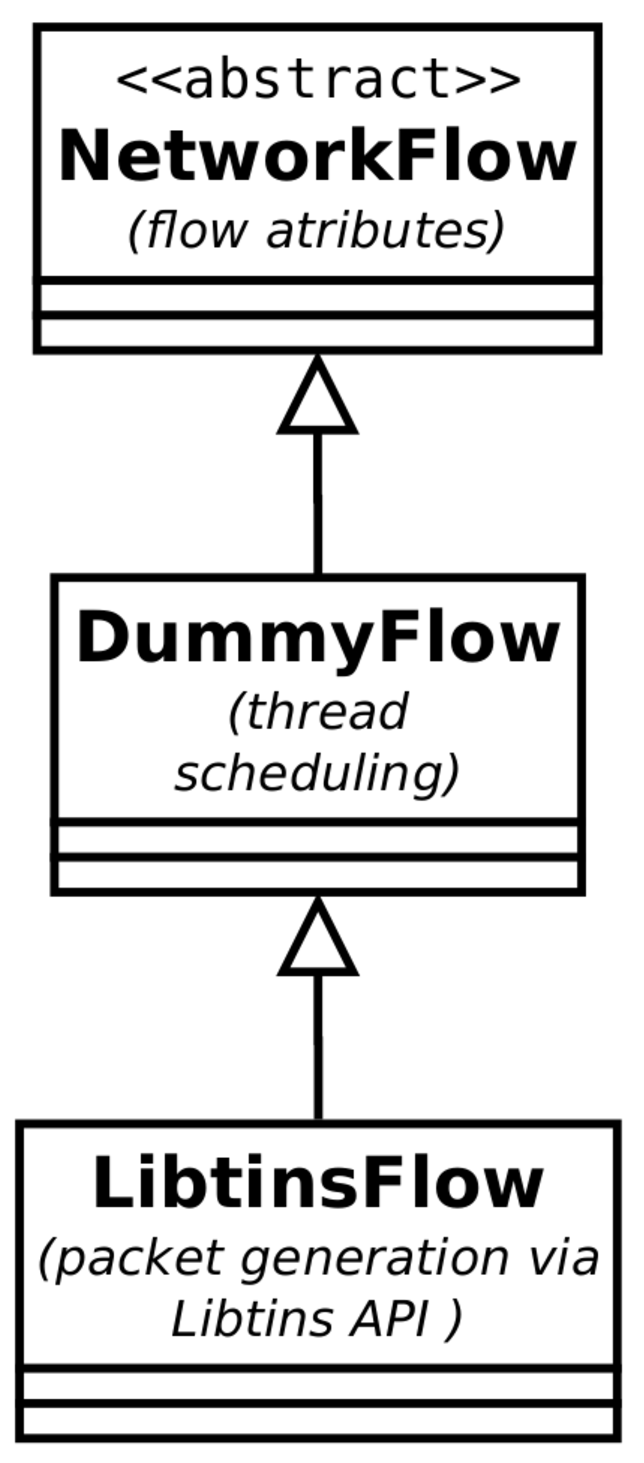
\includegraphics[height=2.0in]{figures/ch6/libtins-flow}
	\caption{Expansion of SIMITAR using Libtins for traffic generation}
	\label{fig:libtins-flow}
\end{figure}

\subsubsection{Traffic generation performance}


\begin{figure}[h!]
	\centering
	\subfloat[DpdkFlow]{
		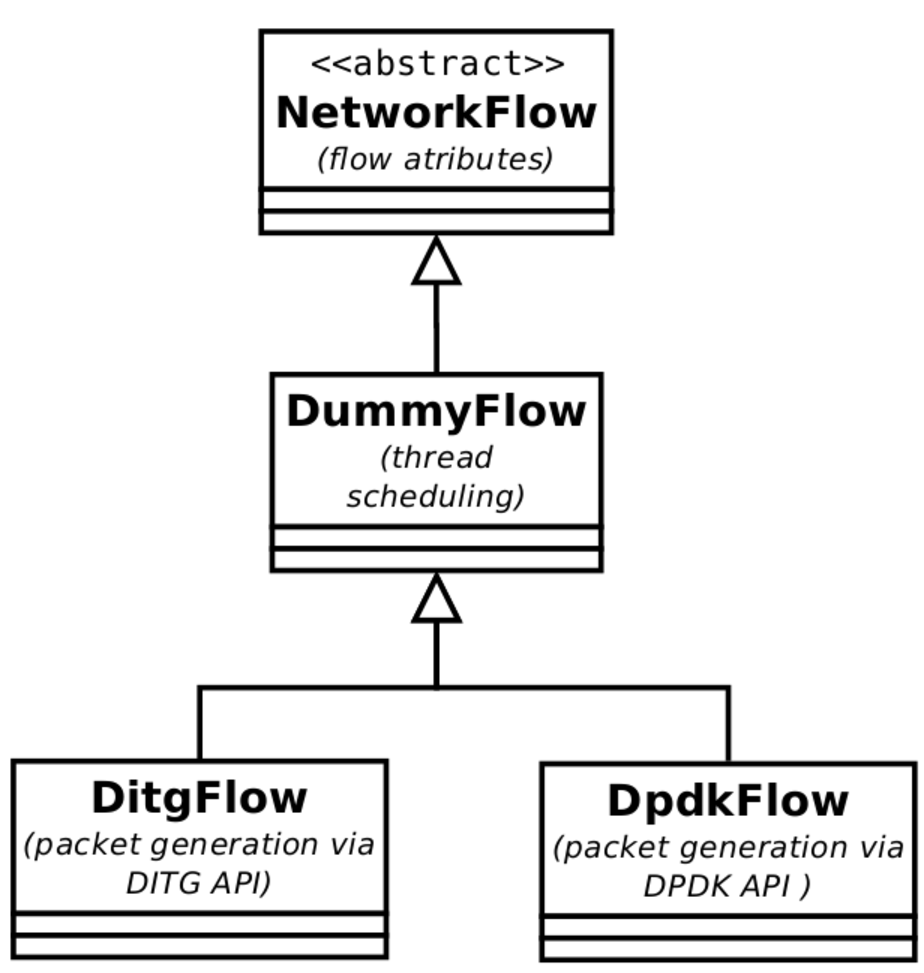
\includegraphics[height=2.0in]{figures/ch6/dpdk-flow}
		\label{fig:dpdk-flow}
	}
	\hspace{0mm}
	\subfloat[DpdkInterface]{
		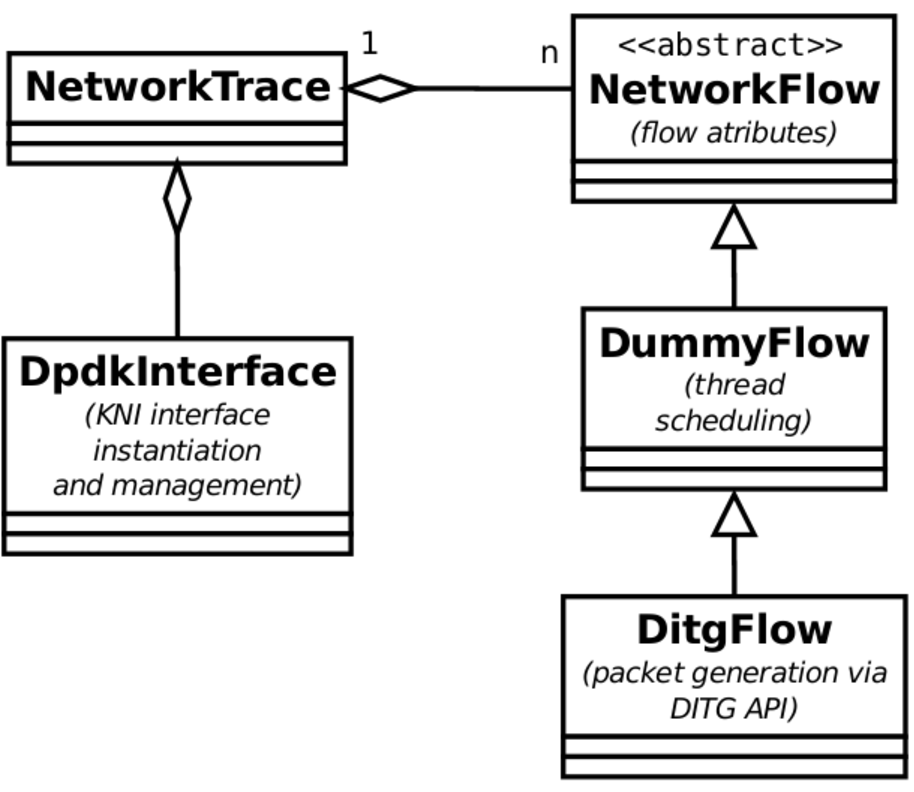
\includegraphics[height=2.0in]{figures/ch6/dpdk-interface}
		\label{fig:dpdk-if}
	}
	\caption{Class diagram for DPDK support expansions. On (a), we have a implementation of traffic generation based on DPDK. On (b) we are using DPDK KNI interfaces.}
	\label{fig:DpdkFlow}
\end{figure}

Some approaches may be taken to improve the traffic generation performance. One possibility is to use DPDK KNI interfaces \footnote{\href{http://dpdk.org/doc/guides/prog_guide/kernel_nic_interface.html}{http://dpdk.org/doc/guides/prog\_guide/kernel\_nic\_interface.html}}. The The DPDK Kernel NIC Interface (KNI) allow applications from the user's space interact with DPDK ports. In this way, we may achieve a faster packet processing. 

Another possibility is to use DPDK API craft packets. Using a low-level library such for packet generation, we will be able to custom generate packets and bypass the Linux network stack (packet acceleration). We present in the figure ~\ref{fig:DpdkFlow} how we could expand our tool to implement a packet generator based on DPDK.


\subsubsection{Thread Menager}

Instead of each flow's thread control individually sleep and wake times, a better approach would be a separated thread control and manage all the other threads' life-cycle operation. This approach can increase the timing accuracy for flows and \textit{files}.


% \subsubsection{Improving DataProcessor Performance}

% Melhorar os algoritimos adicionando técnicas adicionais de modelagem, como condição de parada para o algoritimo gradient descendent, stochastic gradient descendent, entre outros


\subsection{Further Implementations}


\begin{itemize}
	
	\item \textbf{C++ Sniffer}: Implementing the Sniffer and its SQL queries in C++ should increase its performance.
	
	\item \textbf{Use OpenDayLight REST API for data collection}: Another different approach for data collection could be the use the OpenDayLight REST API to collect data from an SDN OpenFlow switches, instead of a using a Sniffer. Through REST API is possible to extract many statistics from nodes, hosts, and ports, such active flows, the number of packets matched per flows, packet drops, and so on. But, different features would be measured,  and a new model for traffic generation would be needed. On the other hand, we could reuse many procedures implemented.  
	
	\item \textbf{SIMITAR Python API}: Currently, SIMITAR only enables the programming of flow traffic generation in C++. Adding Python support for reading NetwrokTrace and NetworkFlow objects, we can enable expansion for Python traffic generation APIs, without creating C++ "wrappers".
	
	\item \textbf{Expand SIMITAR}: Expand the SIMITAR support for more traffic generator tools and APIs, such as MoonGen LUA API, Ostinato Python API, Seagull traffic generator, and many others.
	
	\begin{figure}[!ht]
		\centering
		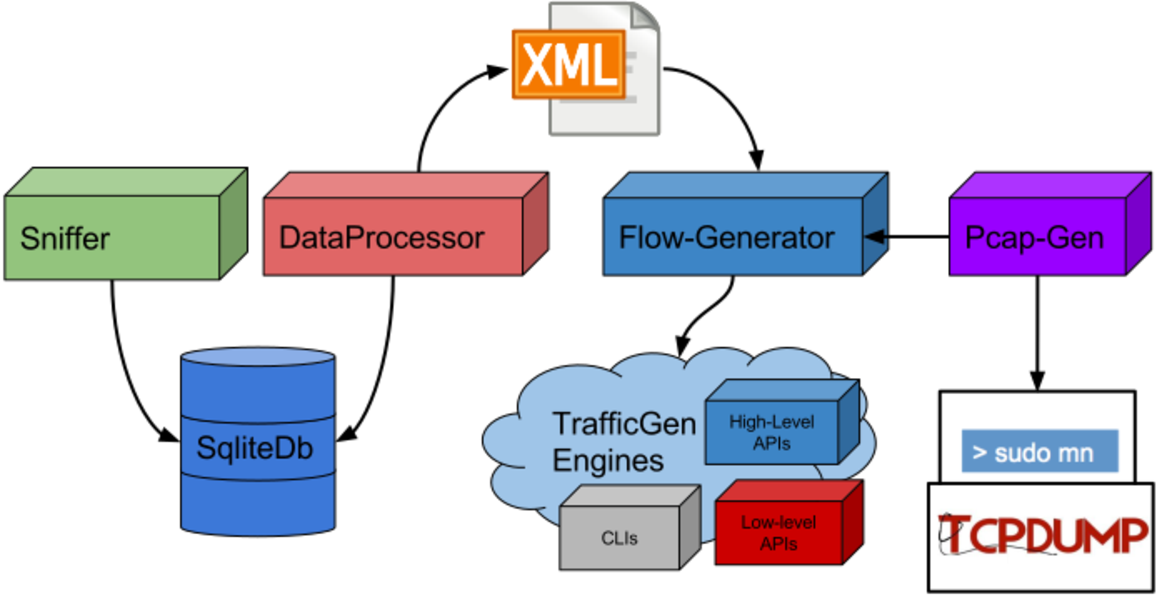
\includegraphics[height=2.0in]{figures/ch6/pcap-gen}
		\caption{Using SIMITAR for generation synthetic \textit{pcap} files, CTD files: a component schema}
		\label{fig:pcap-gen}
	\end{figure}
	
	\item \textbf{PcapGen: a compact \textit{pcap} lybrary}: Create a component capable of generate synthetic \textit{pcap} files, using Compact Trace Descriptors(CTDs) files. We can implement this using SIMITAR as a packet injector, but in an emulated host interface, for example, using Mininet. Then, the traffic can be collected, using a tool such as TCPDump or Tshark. We present a diagram of this idea in the figure ~\ref{fig:pcap-gen}. This expansion would enable SIMITAR  to work as trace library for pcap-based benchmark tools.
	
	% Oferecer a possibilidade de automatização de medições e testes extendendo a ferramenta
	
	% usar redes neurais para classificação de aplicações
	
\end{itemize}










